\chapter{Results and Discussion}
\label{chap:five}
In this section we will discuss the results obtained from 
the performed experiments. We particularly discuss the 
overfitting phenomenon, which is a common problem
for small sample sizes and for low signal to noise problems. 


\section{Results Intepretation}
\label{sec:results}

In this section we will discuss the results obtained from 
the performed experiments. We Particularly discuss the 
overfitting phenomenon, which is a common problem
for small samle sizes. 

\begin{figure}[!h]
    \centering
    \caption{Correlation matrix of the BTC dataset shows high level of 
    multicollinearity.}
    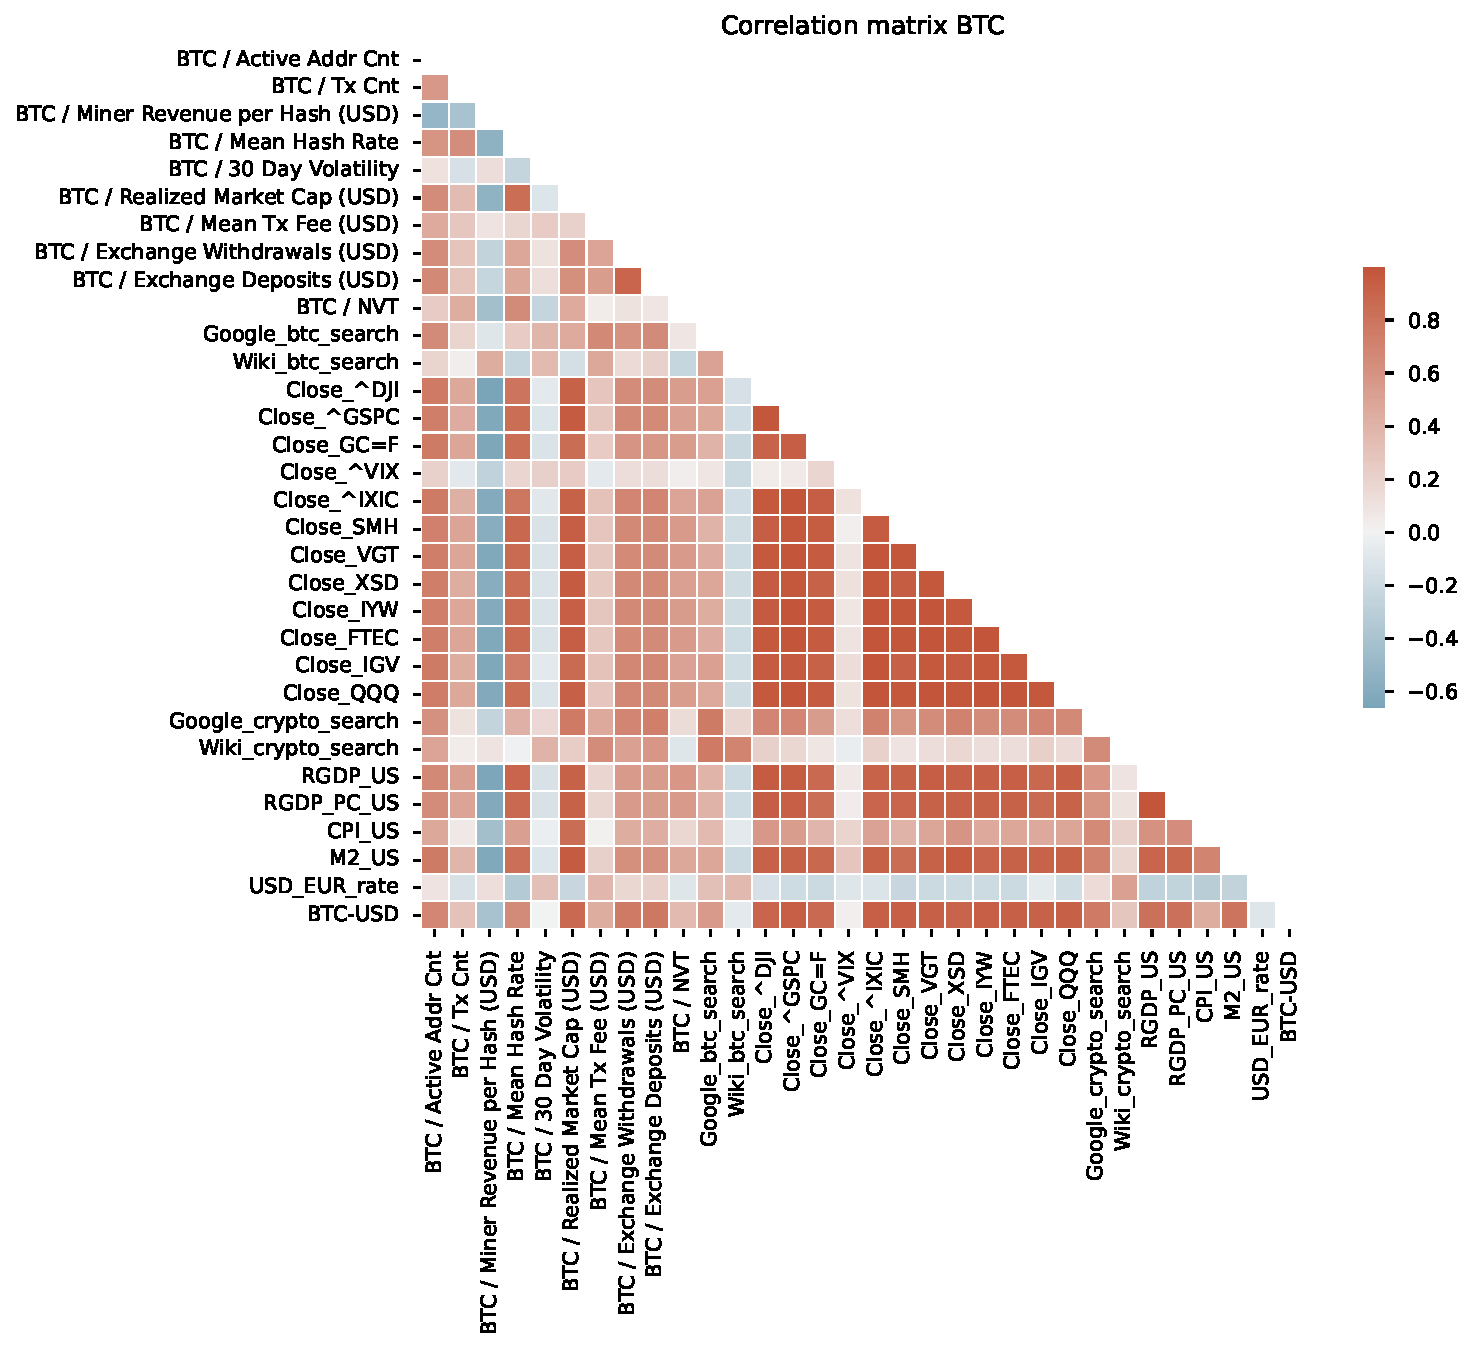
\includegraphics[width=1\textwidth]{Figures/Corr_btc.pdf}
    \caption*{Source: Author}
    \label{fig:Corr_btc}
\end{figure}

\begin{figure}[!h]
    \centering
    \caption{Correlation matrix of the BTC dataset after
    log differencing all of the variables.}
    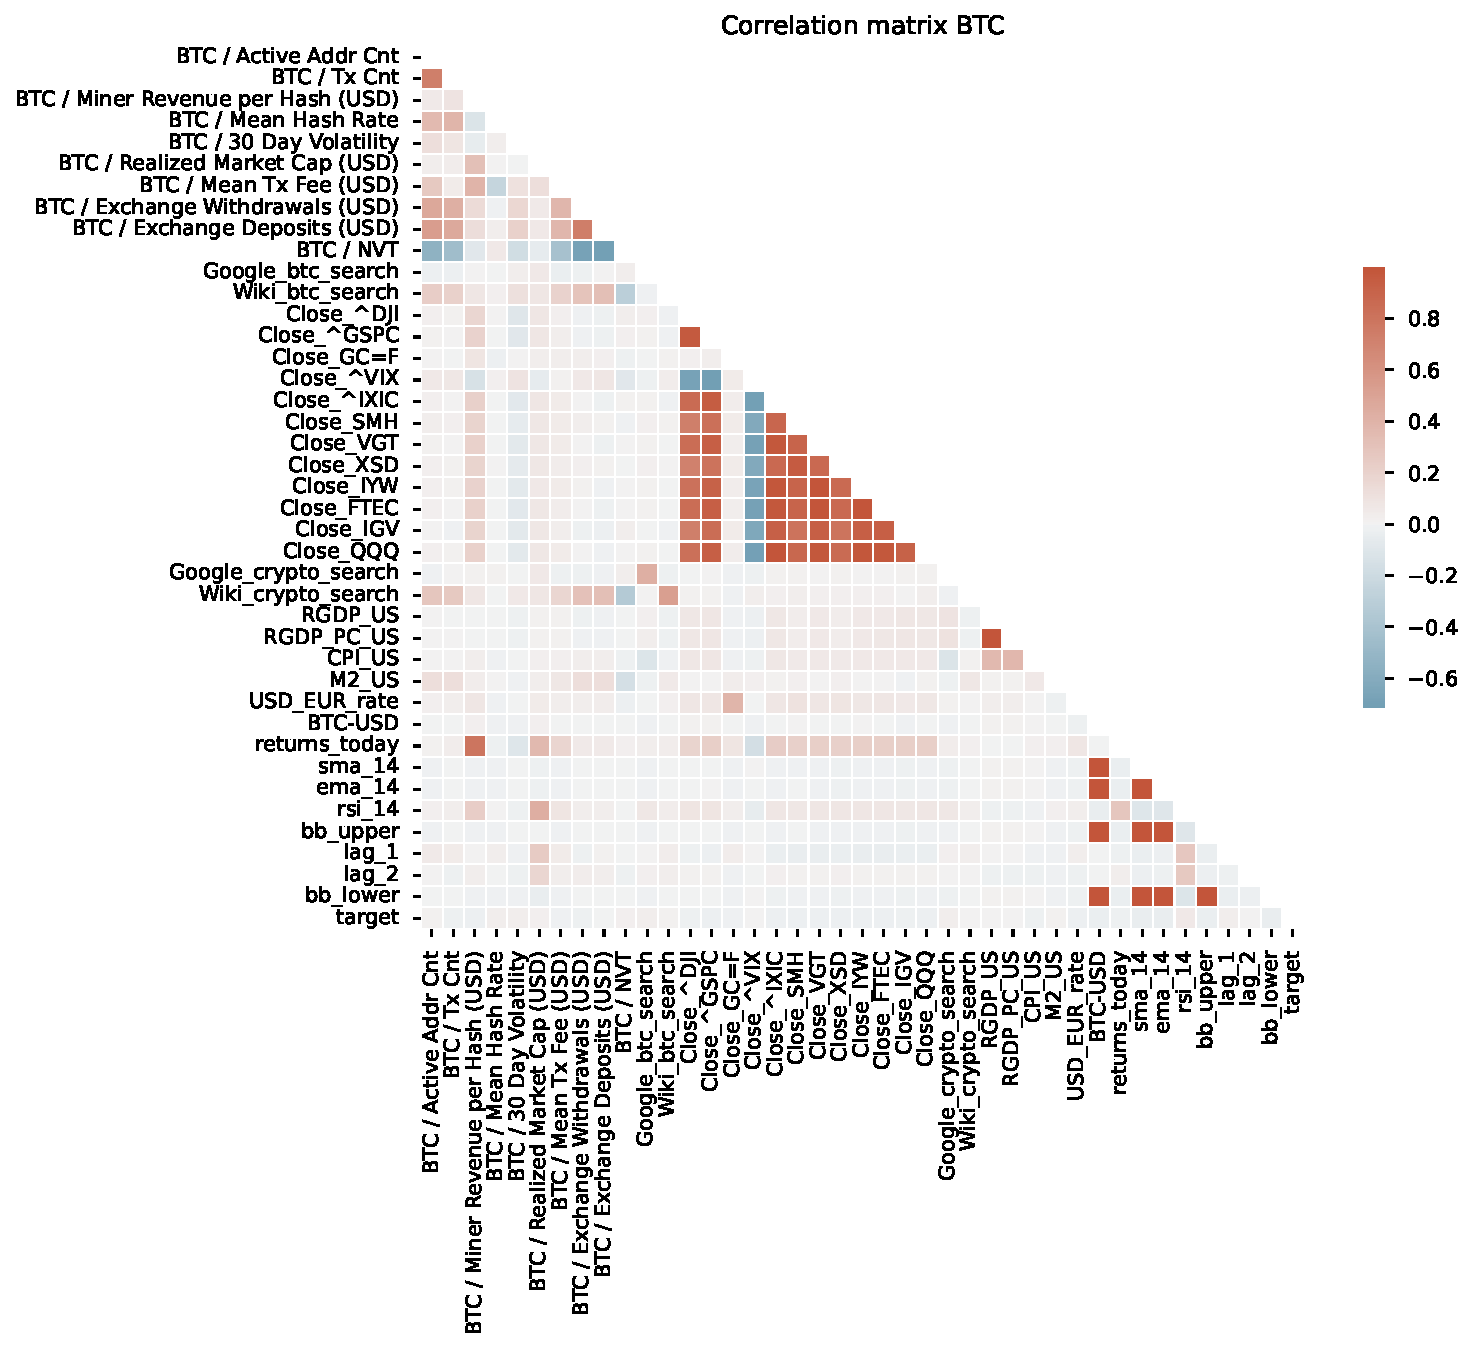
\includegraphics[width=1\textwidth]{Figures/Corr_btc_logdiff.pdf}
    \caption*{Source: Author}
    \label{fig:Corr_btc_logdiff}
\end{figure}




\begin{figure}[!h]
    \centering
    \caption{Learned coefficients of the Ridge regression model
    with incremental training on the BTC dataset. Five 
    coefficients with highest variance are highlighted.}
    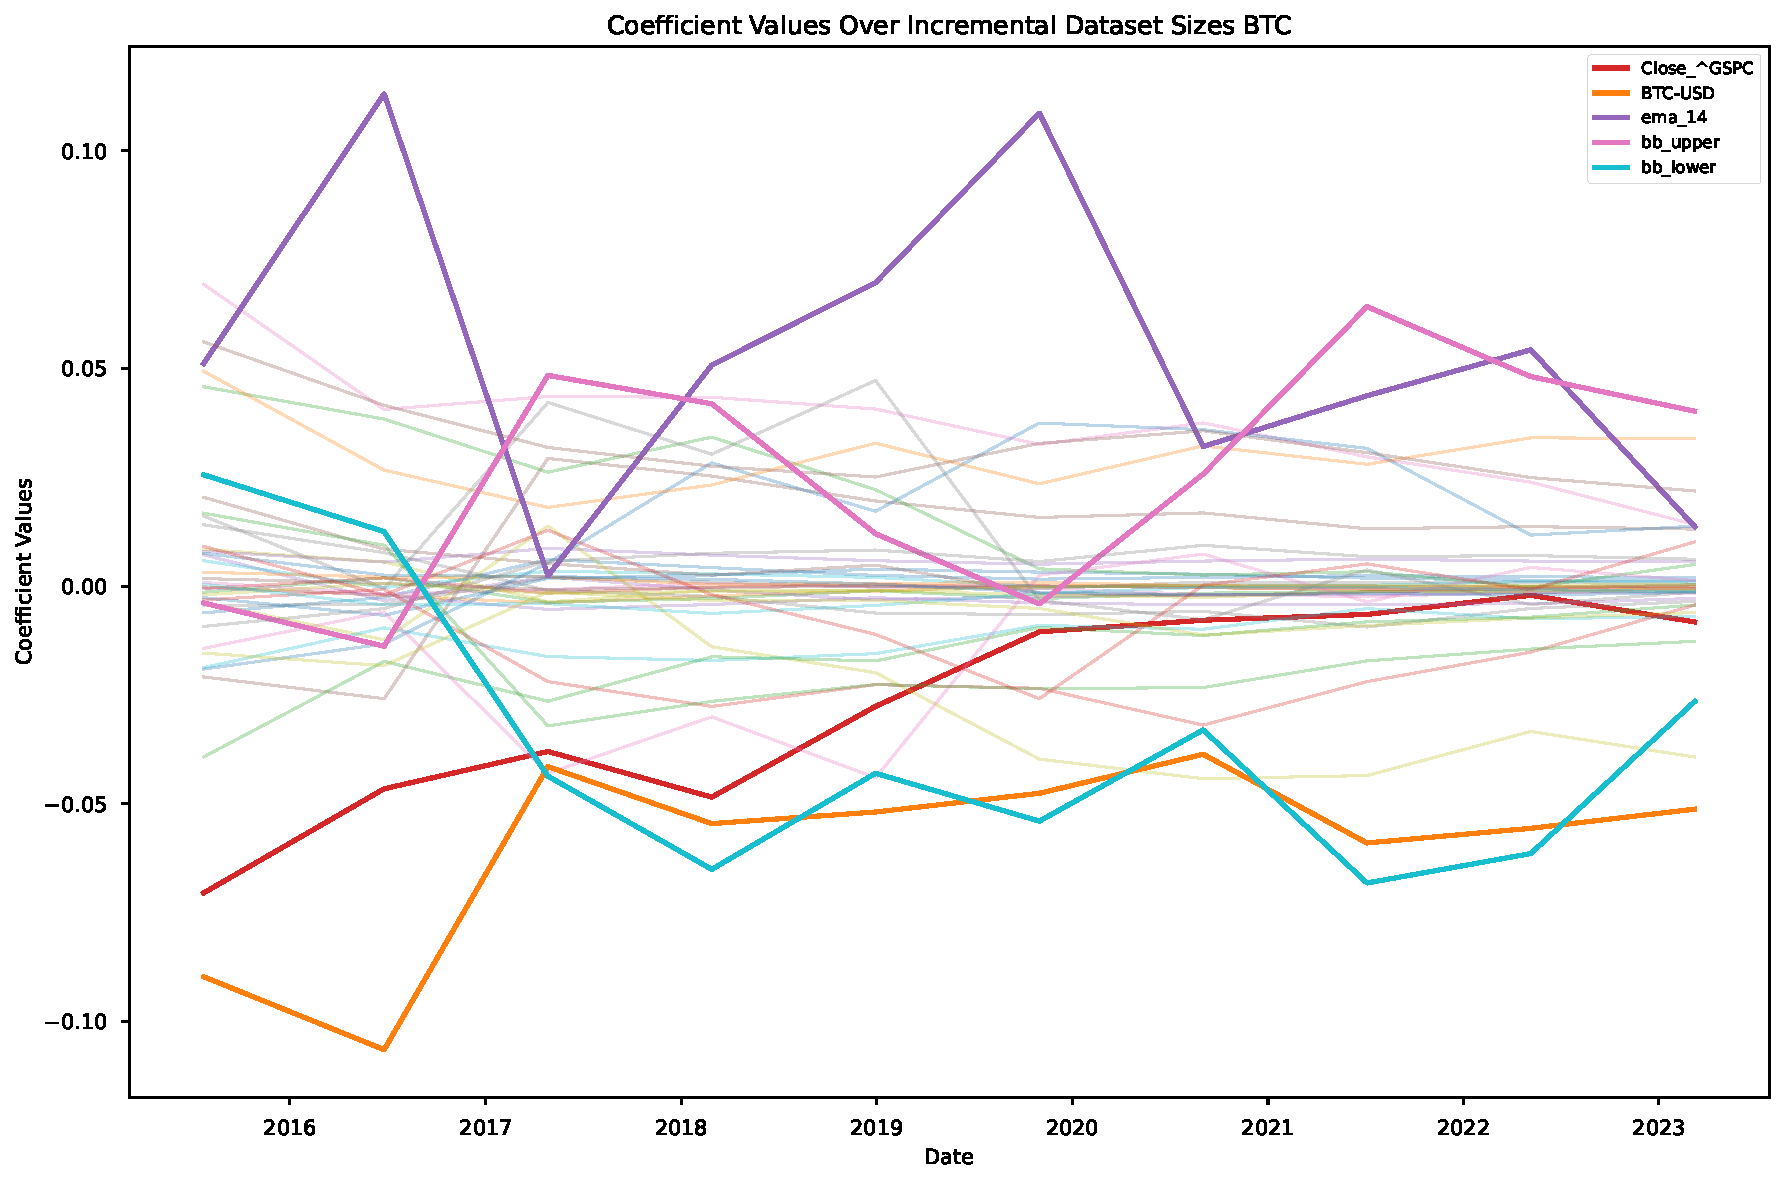
\includegraphics[width=1\textwidth]{Figures/coefficient_values_incremental_btc.pdf}
    \caption*{Source: Author}
    \label{fig:coefs_incremental_btc}
\end{figure}

\begin{figure}[!h]
    \centering
    \caption{Learned coefficients of the Ridge regression model
    with sliding window training on the BTC dataset. Five 
    coefficients with highest variance are highlighted.}
    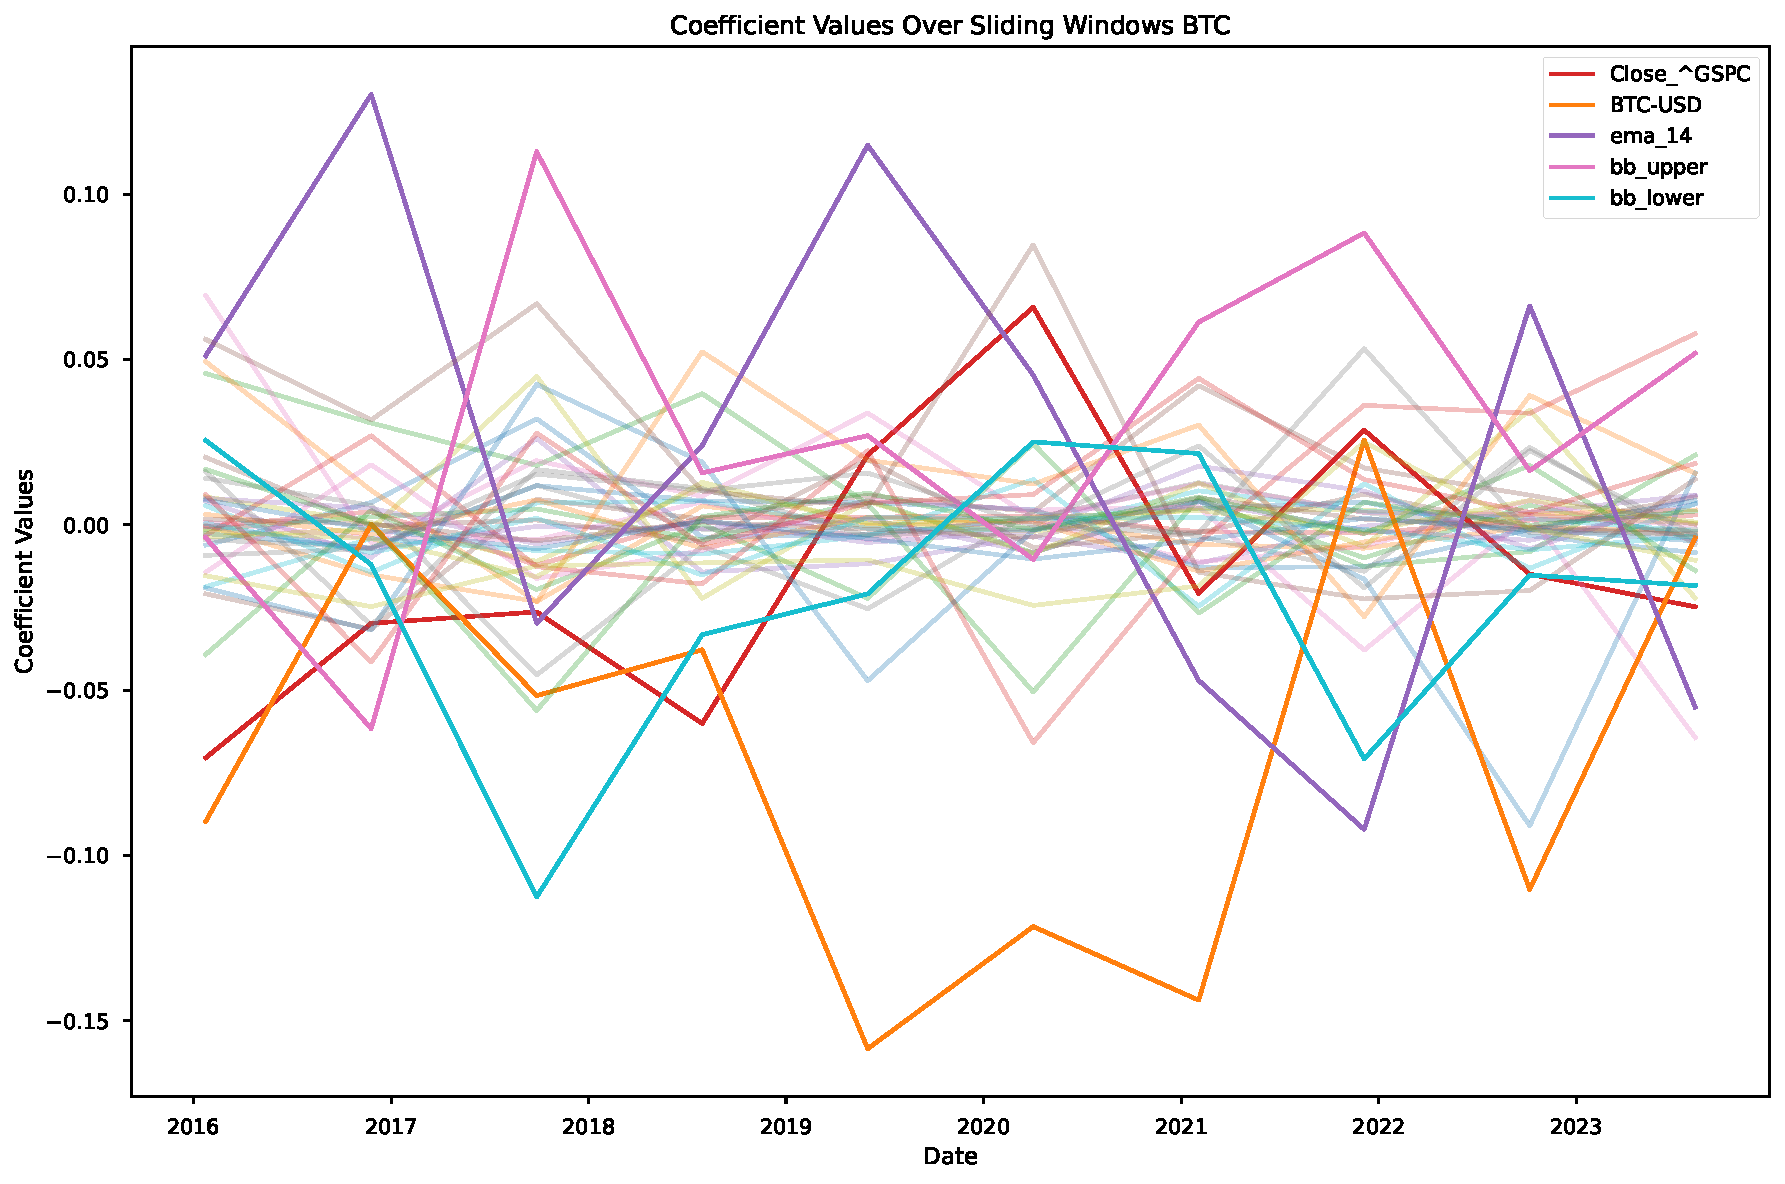
\includegraphics[width=1\textwidth]{Figures/coefficient_values_sliding_btc.pdf}
    \caption*{Source: Author}
    \label{fig:coefs_sliding_btc}
\end{figure}

\section{Limitations}
\label{sec:limitations}
